\documentclass{article}

\usepackage{graphicx}
\usepackage{rotating}
\usepackage{amsmath}
\usepackage{fancyhdr}
\usepackage{listings}
\usepackage{xcolor}
\usepackage{color}
\usepackage{textcomp}
\usepackage{float}
\usepackage{multirow}
\usepackage[sorting=none]{biblatex}
\usepackage[margin=1in]{geometry}
\usepackage[font={small,it}]{caption}
\usepackage{placeins}
\usepackage{xepersian}

%\DeclareMathOperator*{\btie}{\bowtie}
\addbibresource{bibliography.bib}
\settextfont[Scale=1.2]{B-NAZANIN.TTF}
\setlatintextfont[Scale=1]{Times New Roman}
\renewcommand{\baselinestretch}{1.5}
\pagestyle{fancy}
\fancyhf{}
\rhead{تکلیف چهارم درس مبانی بینایی کامپیوتر}
\lhead{\thepage}
\rfoot{علیرضا ابره فروش}
\lfoot{9816603}
\renewcommand{\headrulewidth}{1pt}
\renewcommand{\footrulewidth}{1pt}
%%%%%%%%%%
\lstset
{
    language=[latex]tex,
    basicstyle=\ttfamily,
    commentstyle=\color{black},
    columns=fullflexible,
    keepspaces=true,
    upquote=true,
    showstringspaces=false,
    morestring=[s]\\\%,
    stringstyle=\color{black},
}
%%%%%%%%%%
%beginMatlab
\definecolor{mygreen}{RGB}{28,172,0} % color values Red, Green, Blue
\definecolor{mylilas}{RGB}{170,55,241}
%endMatlab
\begin{document}
%beginMatlab
\lstset{language=Matlab,%
    %basicstyle=\color{red},
    breaklines=true,%
    morekeywords={matlab2tikz},
    keywordstyle=\color{blue},%
    morekeywords=[2]{1}, keywordstyle=[2]{\color{black}},
    identifierstyle=\color{black},%
    stringstyle=\color{mylilas},
    commentstyle=\color{mygreen},%
    showstringspaces=false,%without this there will be a symbol in the places where there is a space
    numbers=left,%
    numberstyle={\tiny \color{black}},% size of the numbers
    numbersep=9pt, % this defines how far the numbers are from the text
    emph=[1]{for,end,break},emphstyle=[1]\color{red}, %some words to emphasise
    %emph=[2]{word1,word2}, emphstyle=[2]{style},    
}
%endMatlab
\begin{titlepage}
\begin{center}

\includegraphics[width=0.4\textwidth]{figures/IUT Logo.png}\\
        
\LARGE
\textbf{دانشگاه صنعتی اصفهان}\\
\textbf{دانشکده مهندسی برق و کامپیوتر}\\
        
\vfill
        
\huge
\textbf{عنوان: تکلیف چهارم درس ریزپردازنده}\\
        
\vfill
        
\LARGE
\textbf{نام و نام خانوادگی: علیرضا ابره فروش}\\
\textbf{شماره دانشجویی: 9816603}\\
\textbf{نیم\,سال تحصیلی: پاییز 1400}\\
\textbf{مدرّس: دکتر عارف کریمی افشار}\\
\end{center}
\end{titlepage}


%\tableofcontents
\newpage


\section{}%1
\subsection{\lr{Prewitt}}
سطح روشنایی پیکسل‌های \lr{h}، \lr{m} و \lr{r} در تصویر فرضی زیر پس از اعمال یک فیلتر هموارکننده‌ی افقی با وزن‌های $\alpha$، $\beta$ و $\gamma$ (نسبت 1:1:1 وزن‌ها (متناظر فیلتر \lr{Prewitt} در جهت افقی) و نسبت 1:2:1 (متناظر فیلتر \lr{Sobel} در جهت افقی) حالات خاص هستند) به ترتیب برابر است با
$
\alpha g + \beta h + \gamma i
$،
$
\alpha l + \beta m + \gamma n
$
و
$
\alpha q + \beta r + \gamma s
$.
پس از اعمال فیلتر مشتق‌گیر عمودی سطح روشنایی پیکسل \lr{m} برابر است با 
$
\alpha (q - g) + \beta (r - h) + \gamma (s - i)
$. \\
از طرفی با اعمال فیلتر \lr{Prewitt} روی تصویر، مقدار پیکسل \lr{m} برابر با 
$
(q - g) + (r - h) + (s - i)
$
می‌شود. از برابری سطح روشنایی‌های به دست آمده از دو روش نتیجه می‌گیریم که اعمال توالی فیلترهای یک بعدی هموارکننده افقی و بعد مشتق‌گیر عمودی معادل با اعمال فیلتر \lr{Prewitt} در جهت عمودی خواهد بود.
\begin{figure}[H]
    \centering
    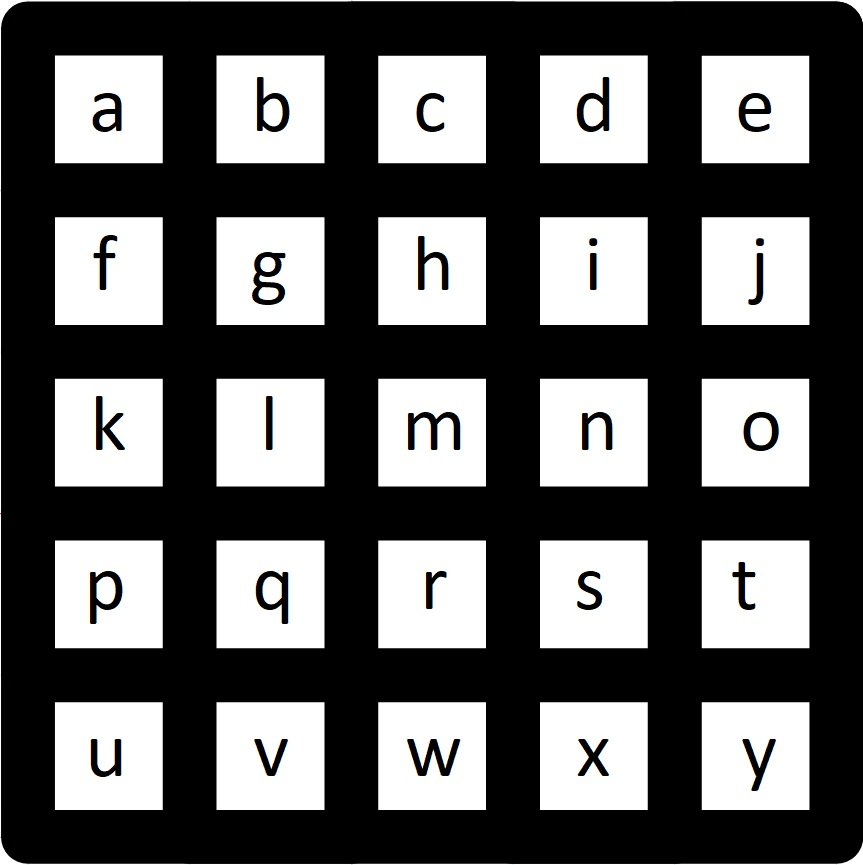
\includegraphics[width=0.5\textwidth]{figures/1p1.jpg}
    \caption
	{}
    \label{fig:fig1}
\end{figure}

\subsection{\lr{Sobel}}
به طریق مشابه سطح روشنایی پیکسل‌های \lr{l}، \lr{m} و \lr{n} در تصویر پس از اعمال یک فیلتر هموارکننده‌ی عمودی با وزن‌های $\alpha$، $\beta$ و $\gamma$ (نسبت 1:1:1 وزن‌ها (متناظر فیلتر \lr{Prewitt} در جهت افقی) و نسبت 1:2:1 (متناظر فیلتر \lr{Sobel} در جهت افقی) حالات خاص هستند) به ترتیب برابر است با
$
\alpha g + \beta l + \gamma q
$،
$
\alpha h + \beta m + \gamma r
$
و
$
\alpha i + \beta n + \gamma s
$.
پس از اعمال فیلتر مشتق‌گیر افقی سطح روشنایی پیکسل \lr{m} برابر است با 
$
\alpha (i - g) + \beta (n - l) + \gamma (s - q)
$. \\
از طرفی با اعمال فیلتر \lr{Sobel} روی تصویر، مقدار پیکسل \lr{m} برابر با 
$
(i - g) + 2 \times (n - l) + (s - q)
$
می‌شود. از برابری سطح روشنایی‌های به دست آمده از دو روش نتیجه می‌گیریم که اعمال توالی فیلترهای یک بعدی هموارکننده عمودی و بعد مشتق‌گیر افقی معادل با اعمال فیلتر \lr{Sobel} در جهت افقی خواهد بود.


\section{}%2





\section{}%3
\subsection{\lr{Algorithm}}
ابتدا 4 گوشه‌ی تصویر را فیکس می‌کنیم. برای پیدا کردن قطعه‌ی متناظر با موقعیت فعلی از میزان شباهت لبه‌ها با یکدیگر استفاده می‌کنیم. برای سنجش شباهت بین دو قطعه از پازل برای همسایگی در یک سطر (ستون)، بردار ویژگی‌های قطعه‌ی سمت چپ (بالا) را برابر سطح روشنایی‌های پیکسل‌های لبه‌ی راست (پایین) و بردار ویژگی‌های قطعه‌ی سمت راست (پایین) را برابر سطح روشنایی‌های پیکسل‌های لبه‌ی چپ (بالا) در نظر می‌گیریم. پیمایش تصویر را از گوشه‌ی چپ و بالا شروع می‌کنیم و توان 2ی فاصله اقلیدسی بردار ویژگی‌های تصویر خاکستری‌گونه‌ی همه‌ی قطعه‌های موجود را با تصویر خاکستری‌گونه‌ی قطعه‌ی فیکس شده حساب می‌کنیم. مینیمم همه این مقادیر مربوط به تصویری است که لبه‌ی آن بیشترین شباهت را از لحاظ سطح روشنایی با لبه‌ی تصویر فیکس شده دارد.
\begin{figure}[H]
    \centering
    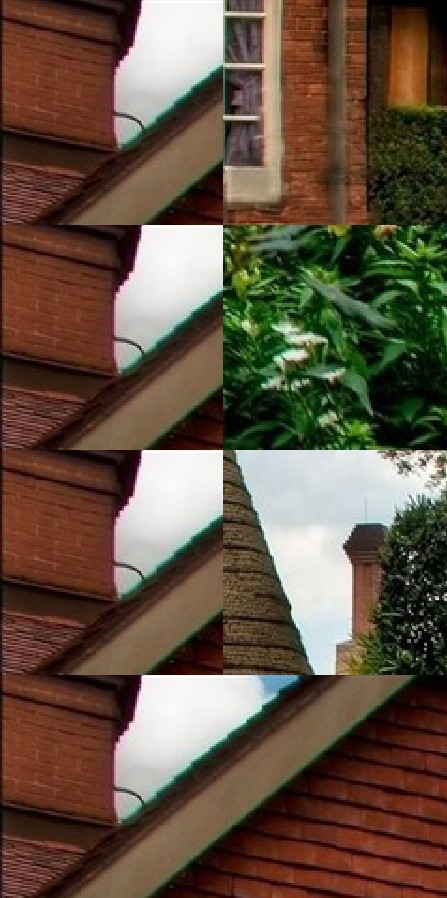
\includegraphics[width=0.5\textwidth]{figures/1p3.jpg}
    \caption
	{
مقایسه‌ی لبه‌ی راست قطعه‌ی گوشه‌ی چپ بالا با چند قطعه
	}
    \label{fig:fig1}
\end{figure}


\begin{figure}[H]
    \centering
    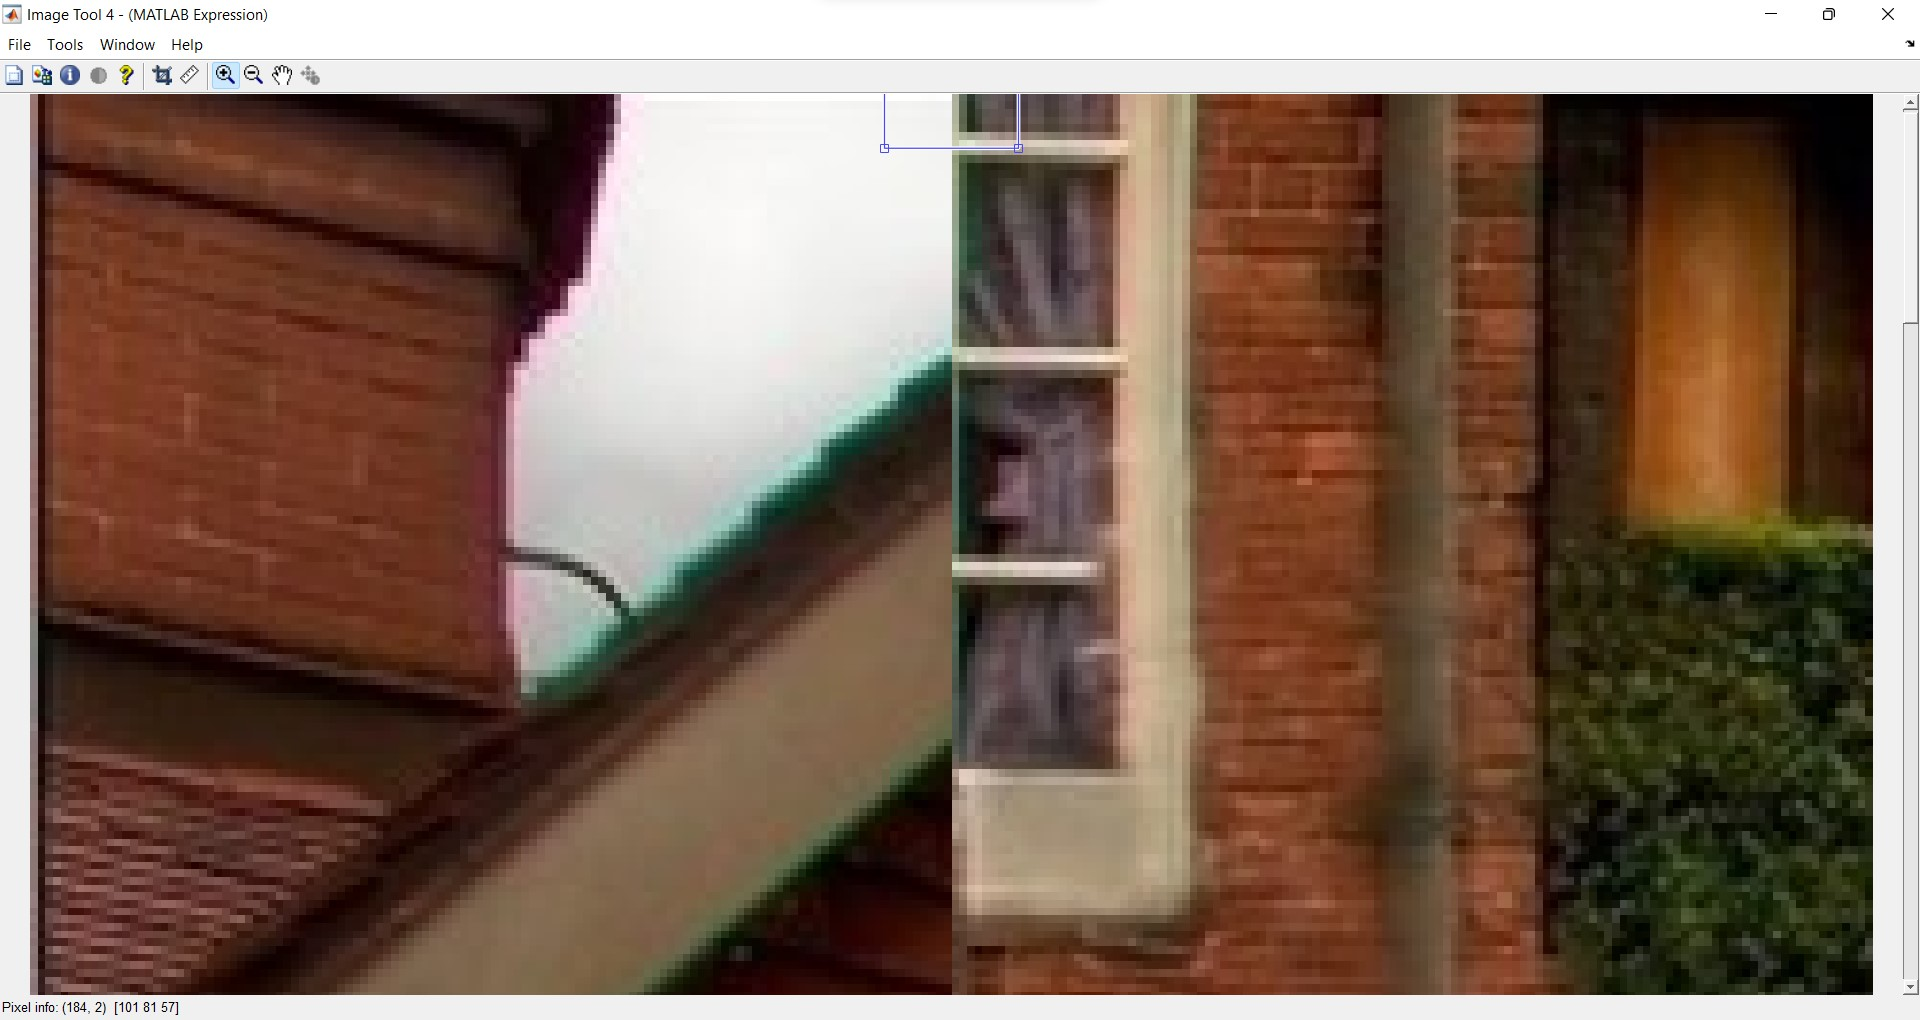
\includegraphics[width=1.0\textwidth]{figures/2p3p.jpg}
    \caption
	{
لبه‌ها (نمای دور)
	}
    \label{fig:fig1}
\end{figure}
\begin{figure}[H]
    \centering
    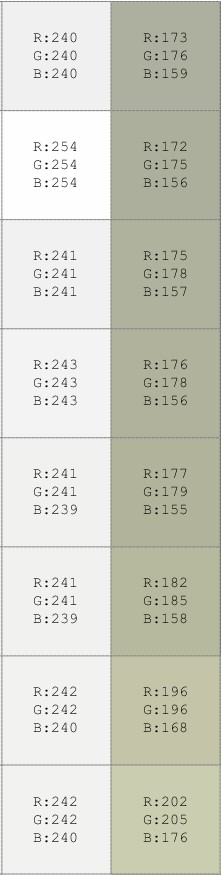
\includegraphics[width=0.25\textwidth]{figures/2p3.jpg}
    \caption
	{
لبه‌ها (نمای نزدیک)
	}
    \label{fig:fig1}
\end{figure}

\begin{figure}[H]
    \centering
    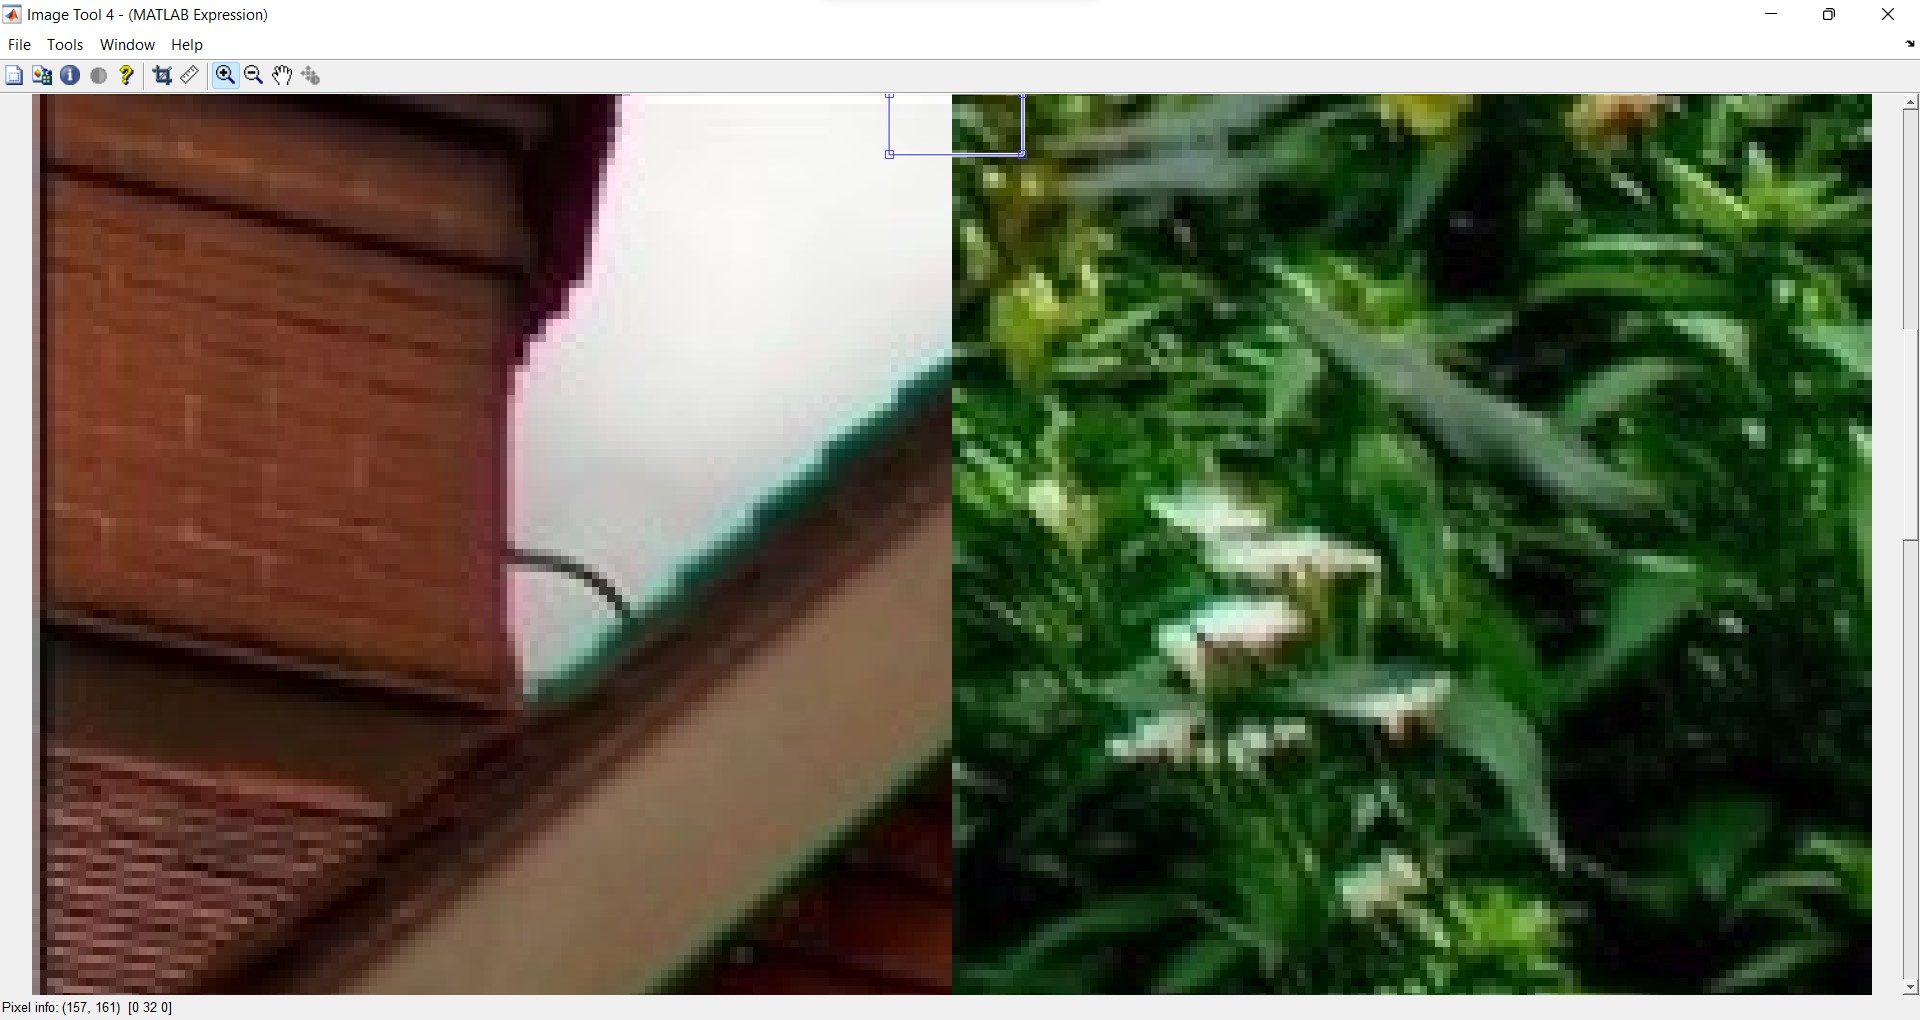
\includegraphics[width=1.0\textwidth]{figures/3p3p.jpg}
    \caption
	{
لبه‌ها (نمای دور)
	}
    \label{fig:fig1}
\end{figure}
\begin{figure}[H]
    \centering
    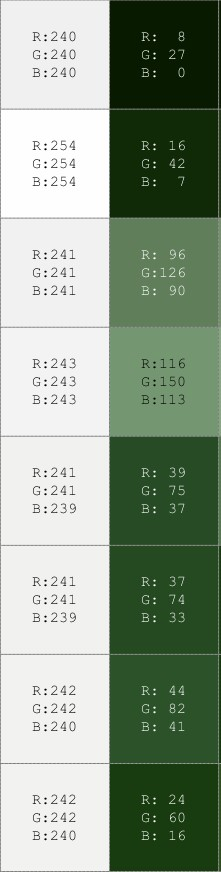
\includegraphics[width=0.25\textwidth]{figures/3p3.jpg}
    \caption
	{
لبه‌ها (نمای نزدیک)
	}
    \label{fig:fig1}
\end{figure}

\begin{figure}[H]
    \centering
    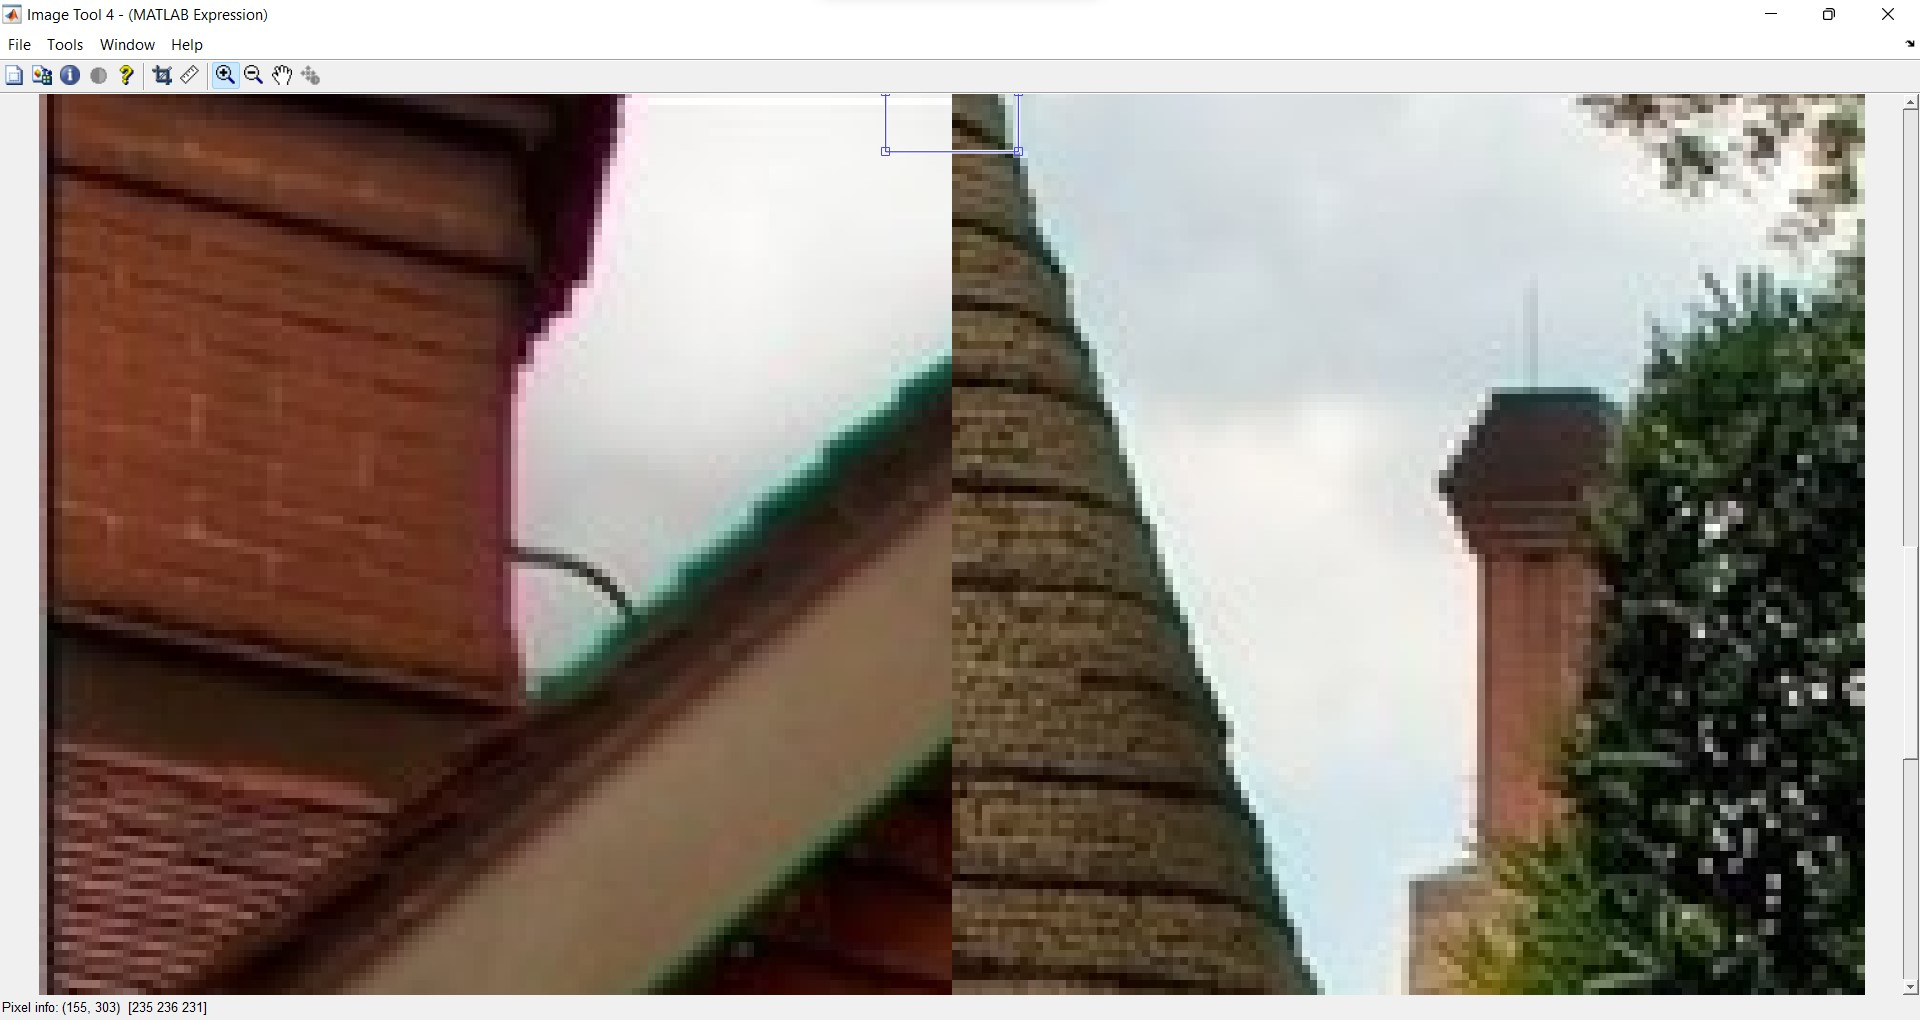
\includegraphics[width=1.0\textwidth]{figures/4p3p.jpg}
    \caption
	{
لبه‌ها (نمای دور)
	}
    \label{fig:fig1}
\end{figure}
\begin{figure}[H]
    \centering
    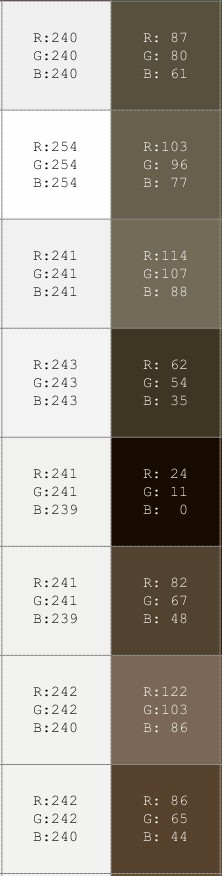
\includegraphics[width=0.25\textwidth]{figures/4p3.jpg}
    \caption
	{
لبه‌ها (نمای نزدیک)
	}
    \label{fig:fig1}
\end{figure}

\begin{figure}[H]
    \centering
    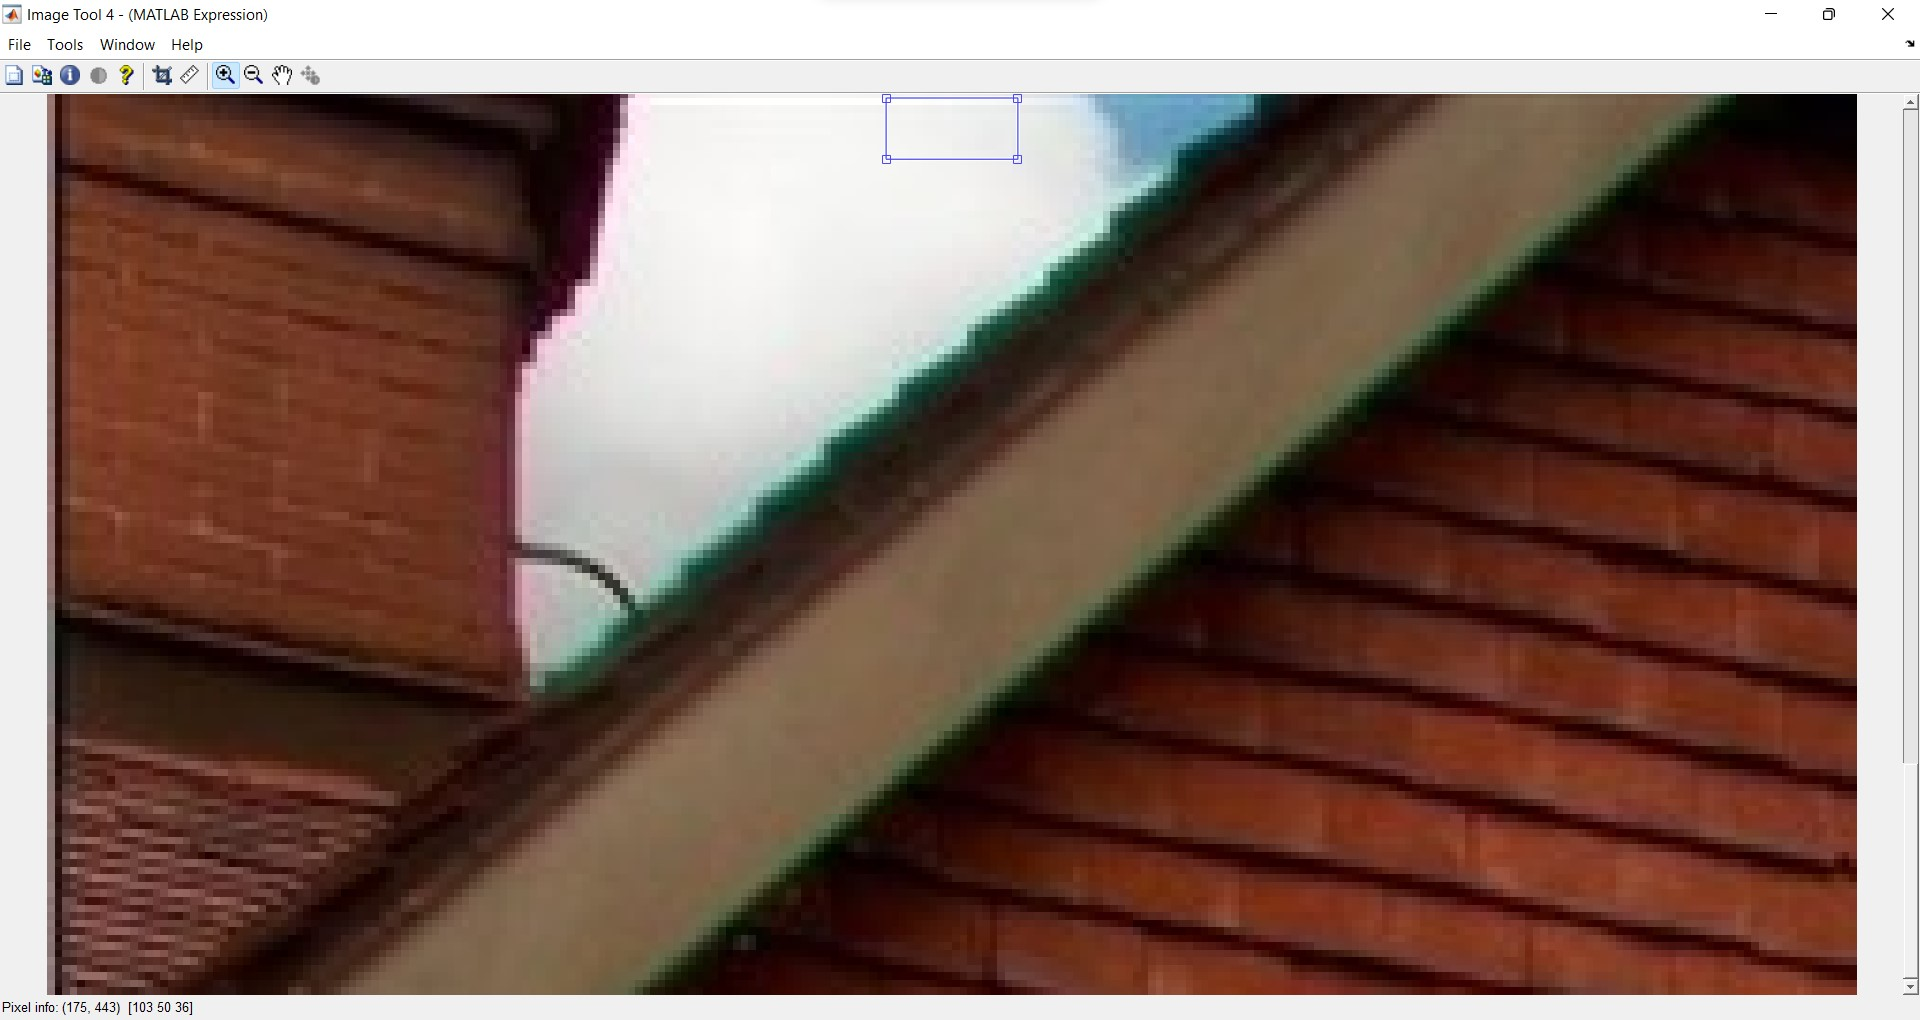
\includegraphics[width=1.0\textwidth]{figures/5p3p.jpg}
    \caption
	{
لبه‌ها (نمای دور)
	}
    \label{fig:fig1}
\end{figure}
\begin{figure}[H]
    \centering
    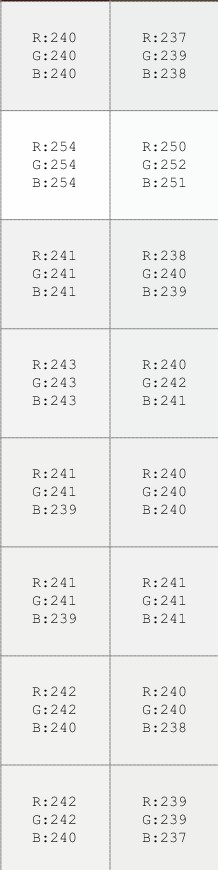
\includegraphics[width=0.25\textwidth]{figures/5p3.jpg}
    \caption
	{
لبه‌ها (نمای نزدیک)
	}
    \label{fig:fig1}
\end{figure}


\subsection{\lr{Function}}
\begin{latin}
\lstinputlisting{sources/borderDiff.m}
\end{latin}

\subsection{\lr{Driver code}}
\subsubsection{الف}
\begin{latin}
\lstinputlisting{sources/p3a.m}
\end{latin}
\subsubsection{ب}
\begin{latin}
\lstinputlisting{sources/p3b.m}
\end{latin}

\subsection{\lr{Results}}
\subsubsection{الف}
\begin{figure}[H]
    \centering
    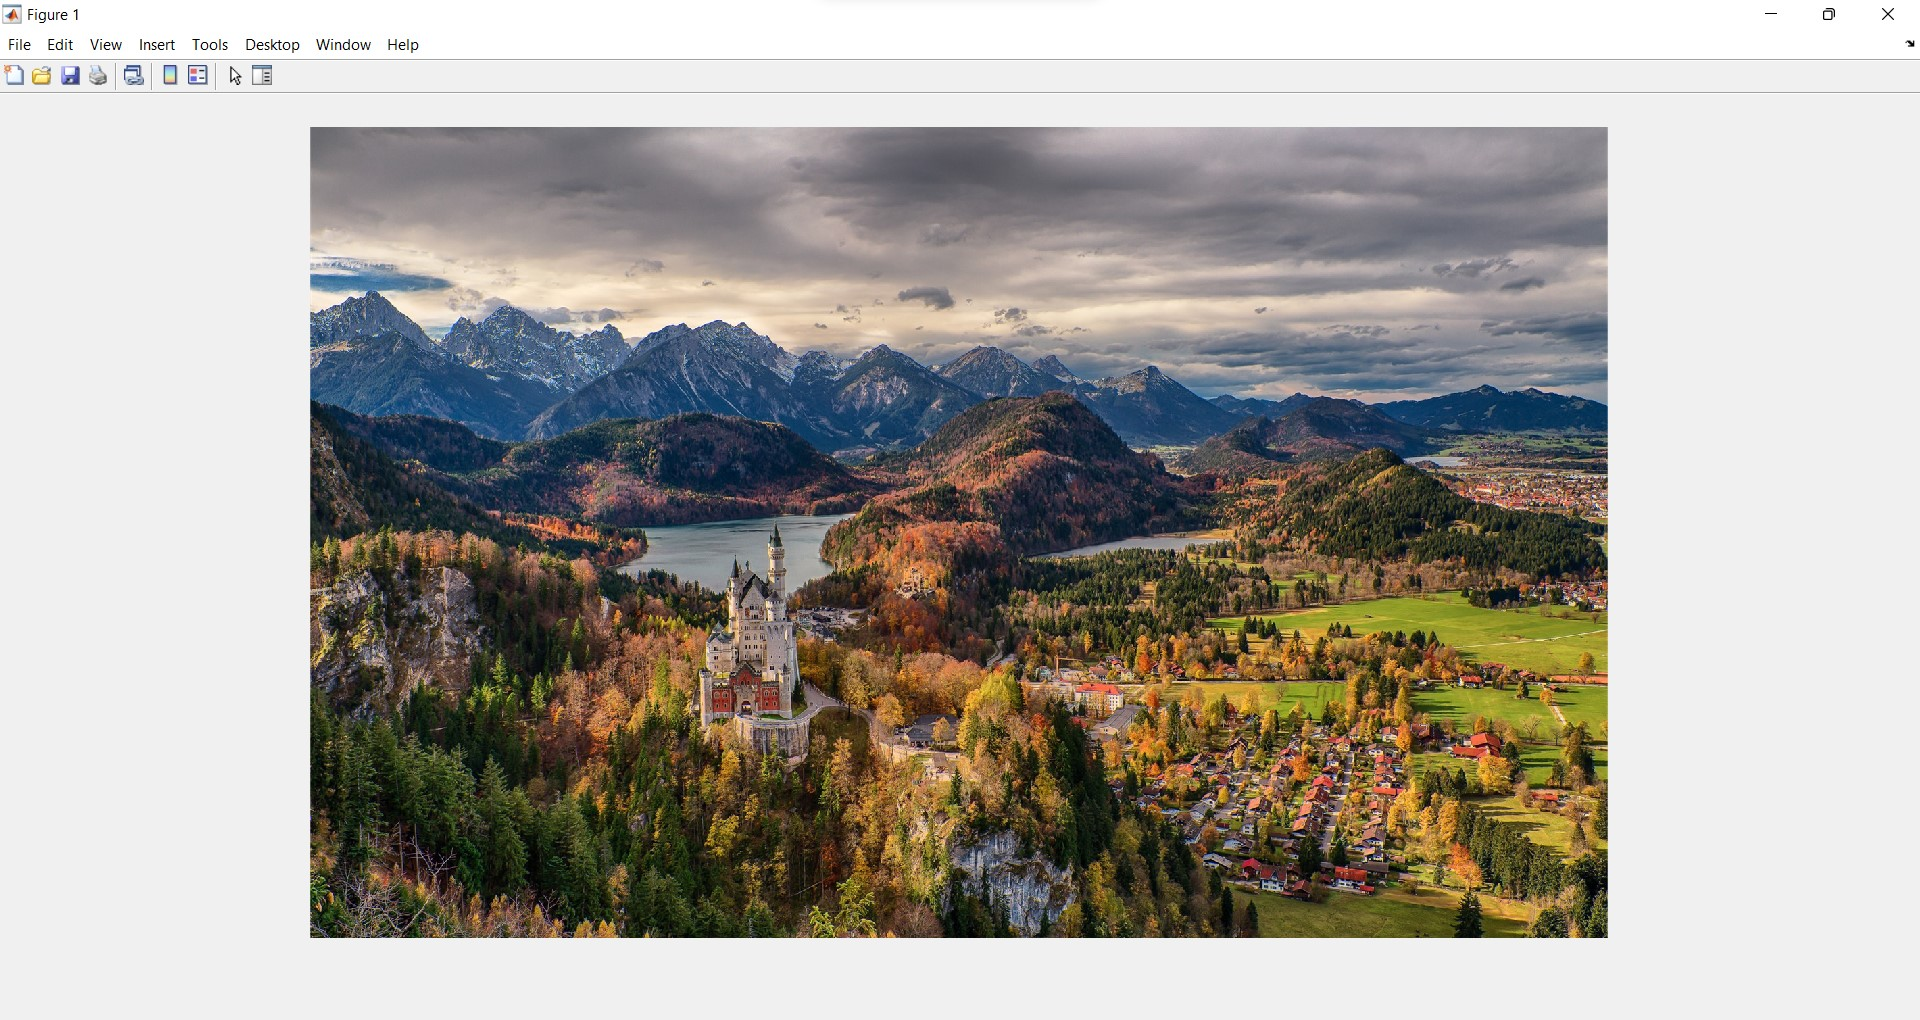
\includegraphics[width=1.0\textwidth]{figures/p3a.jpg}
    \caption
	{}
    \label{fig:fig1}
\end{figure}

\subsubsection{ب}
\begin{figure}[H]
    \centering
    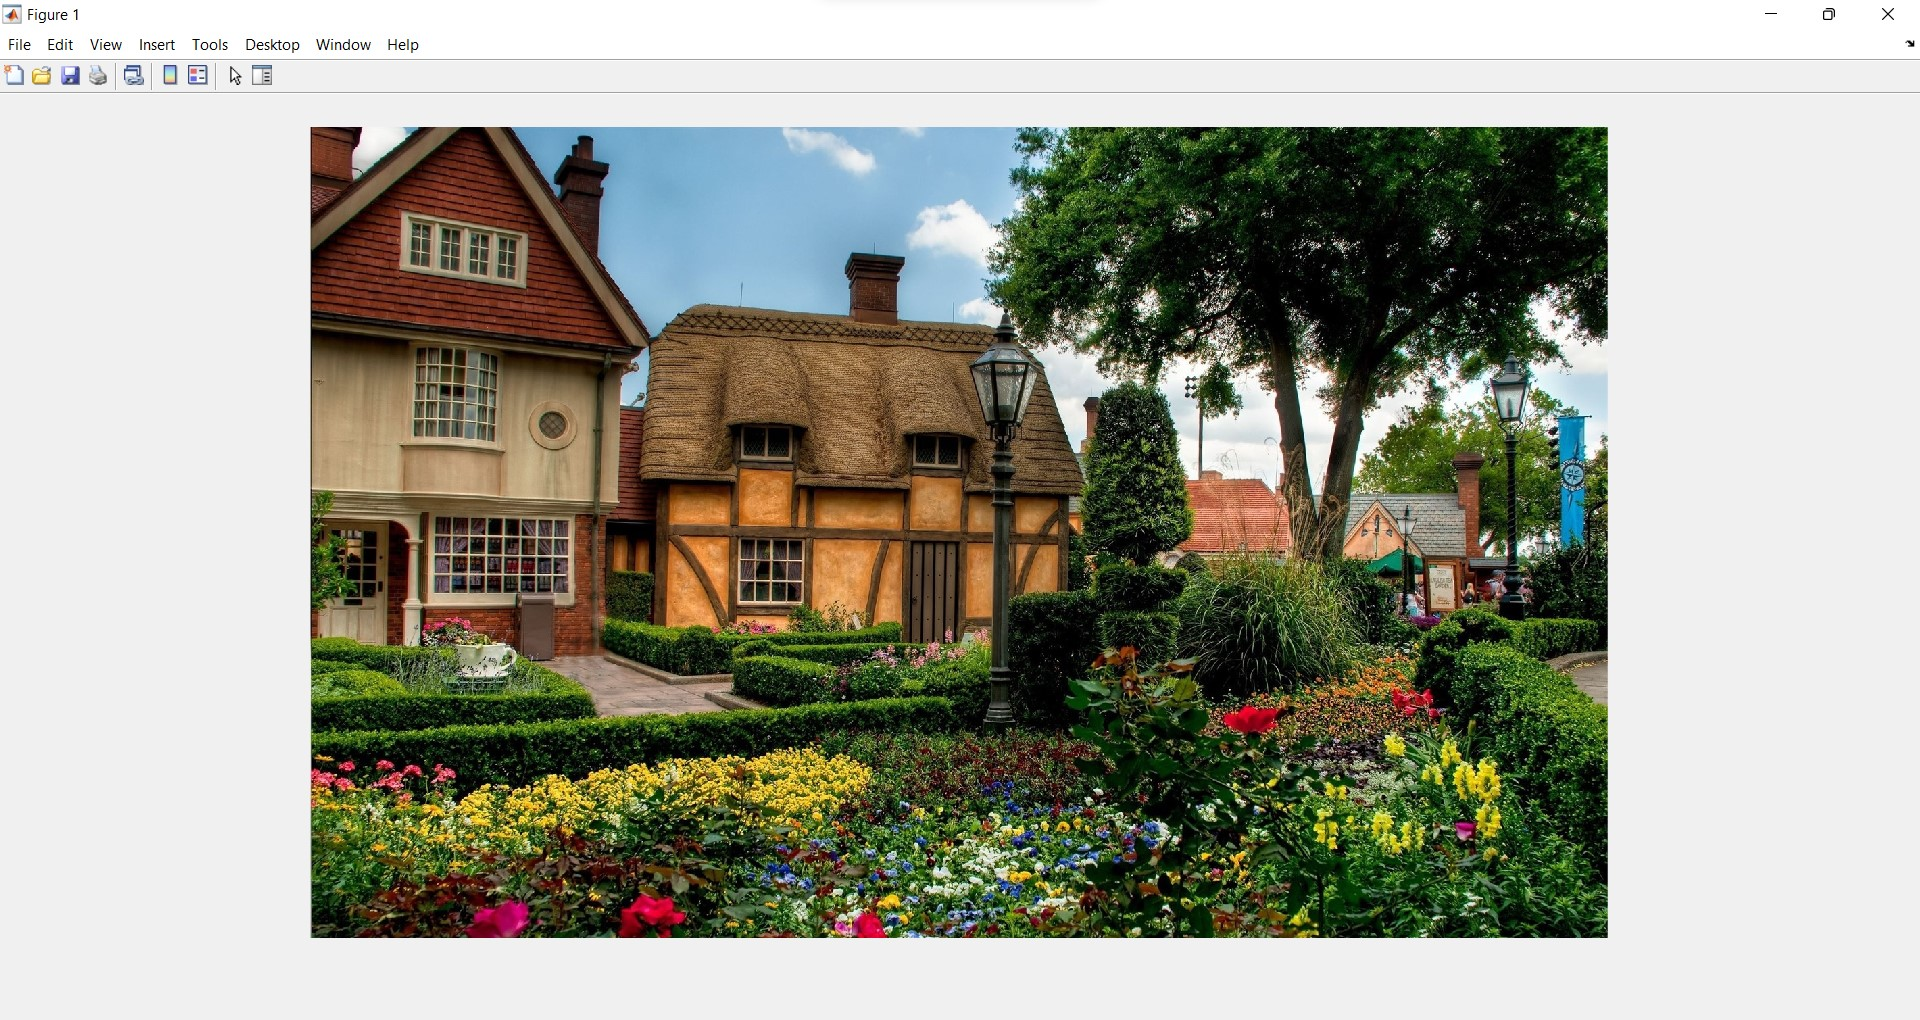
\includegraphics[width=1.0\textwidth]{figures/p3b.jpg}
    \caption
	{}
    \label{fig:fig1}
\end{figure}




%%%%%%%%%%%%%%%%%%%%%%%%%%%%%%%%%%%


%\begin{latin}
%\lstinputlisting{sources/p1.m}
%\end{latin}



%%%%%%%%%%%%%%%%%%%%%%%%%%%%%%%%%%%
%%%%%%%%%%%%%%%%%%%%%%%%%%%%%%%%%%%
%%%%%%%%%%%%%%%%%%%%%%%%%%%%%%%%%%%

%------------------------------------------------------------------------------------------


\section*{منابع}
\renewcommand{\section}[2]{}%
\begin{thebibliography}{99} % assumes less than 100 references
%چنانچه مرجع فارسی نیز داشته باشید باید دستور فوق را فعال کنید و مراجع فارسی خود را بعد از این دستور وارد کنید


\begin{LTRitems}

\resetlatinfont

\bibitem{b1}
\end{LTRitems}

\end{thebibliography}


\end{document}
